%\documentclass[runningheads]{llncs}
% \documentclass[a4paper,12pt]{report}
\documentclass[a4paper,12pt]{article}
%\renewcommand{\baselinestretch}{1.5}
\usepackage{amsmath,amssymb,amsthm}
\renewcommand{\qedsymbol}{$\blacksquare$}
\usepackage{fixltx2e}
\usepackage{amsmath}
\usepackage{graphicx}
\usepackage{color}
\usepackage[utf8]{inputenc}
\usepackage{float}
\usepackage{epstopdf}
\usepackage{lineno}
\usepackage[T1]{fontenc}
\usepackage{ragged2e}
\usepackage{xifthen} 
\usepackage{tabularx}
\usepackage[ruled,vlined]{algorithm2e}
\usepackage{algpseudocode}
\usepackage{subfig} %For SubFigures


\usepackage{algorithm}
\usepackage[noend]{algpseudocode}

\usepackage{listings}
\usepackage{color}

\definecolor{dkgreen}{rgb}{0,0.6,0}
\definecolor{gray}{rgb}{0.5,0.5,0.5}
\definecolor{mauve}{rgb}{0.58,0,0.82}

\lstset{frame=tb,
  language=Matlab,
  aboveskip=3mm,
  belowskip=3mm,
  showstringspaces=false,
  columns=flexible,
  basicstyle={\small\ttfamily},
  numbers=none,
  numberstyle=\tiny\color{gray},
  keywordstyle=\color{blue},
  commentstyle=\color{dkgreen},
  stringstyle=\color{mauve},
  breaklines=true,
  breakatwhitespace=true,
  tabsize=3
}

\newcommand{\mychapter}[2]{
    \setcounter{chapter}{#1}
    \setcounter{section}{0}
    \chapter*{#2}
    \addcontentsline{toc}{chapter}{#2}
}

\newcommand{\oneline}[1]{%
  \newdimen{\namewidth}%
  \setlength{\namewidth}{\widthof{#1}}%
  \ifthenelse{\lengthtest{\namewidth < \textwidth}}%
  {#1}% do nothing if shorter than text width
  {\resizebox{\textwidth}{!}{#1}}% scale down
}

\begin{document}

\begin{titlepage}
\begin{center}
{

\vspace{-1cm}
    \LARGE
    \textbf{Software Component Identification and Composition}

\vspace{1cm}
    \large
    \textbf{State of the Art Report}\\[1cm]
    \oneline{\large{Submitted in Partial Fulfillment of Requirements for the Degree of}}
    \\[0.5cm]
    {Masters of Technology}

\vspace{1cm}
\normalsize
By\\
{\large
\textbf{Anshuman Sekhar Dash\\
M.Tech. 3\textsuperscript{rd} Sem\\
Information Security\\
Reg No: 2020IS04}
}\\[1cm]

{\large 
Under the Supervision of\\
\textbf{Prof. D. K. Yadav}
}\\[1cm]

\includegraphics[width=3.5cm]{logo.jpeg}\\[1cm]

\oneline{\Large \textbf{Computer Science \& Engineering Department}}\\
\oneline{\Large \textbf{Motilal Nehru National Institute of Technology Allahbad}}\\
\oneline{\Large \textbf{Prayagraj, India}}

}
\end{center}
\end{titlepage}

\pagenumbering{Roman}

%-----------------------Undertaking --------------------------------------
\newpage
\Huge
\centering \textbf{DECLARATION}\\
\normalsize
\justify
%\vskip2cm	
\vspace{10pt}	\par  I, hereby declare that the work presented in this \textbf{State of the Art}  report  dissertation entitled “Software Component Identification and Composition” has been done by me under the supervision of Prof. D. K. Yadav, and this dissertation embodies my own work.
\vskip5cm
Name : Anshuman Sekhar Dash\\
\vskip.2cm
Registration No. : 2020IS04\\
\vskip.2cm
Date : December 13, 2021
%-----------------------Abstract --------------------------------------
\newpage
\begin{center}{\begin{Large}
\textbf{CERTIFICATE BY EXAMINERS}
\end{Large}}\\
%\vskip1cm
\vskip0.3cm

\includegraphics[height=3cm]{logo.jpeg}\\

\oneline{\Large \textbf{Computer Science \& Engineering Department}}\\
\oneline{\Large \textbf{Motilal Nehru National Institute of Technology Allahbad}}\\
\oneline{\Large \textbf{Prayagraj, India}}
\end{center}

\vskip0.3cm
%\vskip2cm	
\vspace{10pt}
\par This is to certify that the \textbf{State of the Art}  report entitled \textbf{Software Component Identification and Composition} is submitted by ANSHUMAN SEKHAR DASH (Registration No. 2020IS04)  has been examined by the undersigned as a part of the examination and fulfills the requirement of Master  of Technology in Software Engineering,  MOTILAL NEHRU NATIONAL INSTITUTE OF TECHNOLOGY ALLAHABAD.
\vskip4cm
Signature \space\space\space\space\space\space\space\space\space\space\space\space\space\space \space\space\space\space\space\space \space\space\space\space\space\space Signature\space\space\space\space\space\space\space\space\space\space\space\space\space\space\space\space\space\space\space\space\space\space\space\space\space\space Signature 
\vskip 0.5cm
 Name \space\space\space\space\space\space\space\space\space\space\space\space\space\space \space\space\space\space\space\space \space\space\space\space\space\space \space\space\space\space\space\space Name\space\space\space\space\space\space\space\space\space\space\space\space\space\space\space\space\space\space\space\space\space\space\space\space\space\spacepace\space\space\space\space\space Name
\newpage

%-----------------------Abstract --------------------------------------

\Huge
\centering \textbf{Abstract}\\
\normalsize
\justify
Reusing of software is found to have escalate the software engineers work output and
also the craftsmanship of the final software product. Component based software engineering
(CBSE) is a unique area in software engineering wherein software components i.e a chunk of
software that contains a set of related functions and data are searched for and pieced together
to form a software system.This method promotes re usability and efficiency in development
of software systems. CBSE’s purpose is to compose software applications using plug and
play software components on the framework.There are several strategies for software component identification in a system among which most widely used is object oriented based
clustering.we will look into various approaches used in identifying a software component.We propose a approach which is based on clustering and formal methods to solve the problem of software component identification from a software system.The approach is based on describing a software component using formal methods and then using clustering algorithms that will groups the components in an hierarchy.when components are arranged in an hierarchical manners it provides a means to store ,browse and retrieve reusable software components.we will use the software components identified to compose a different system for comparison and demonstration of correctness of our approach used. 
\newpage


%-------------------------------------------

\newpage
\tableofcontents
\newpage
\listoffigures
\cleardoublepage\pagenumbering{arabic}

%-------------------------------------------

\section{Introduction}
% no \IEEEPARstart
\subsection{What is Component Based Software Engineering}
From the last 10 years use of computer software has entered into every part of economy which has in turn generated new demand from the software industry to develop reliable and cost effective software quickly and efficiently.
Modern software systems are becoming more and more large scale which further increases the development cost , decreases the productivity and increases the cost of maintenance.
In the 90's a understanding was developed among software engineers that a software system need not be developed all the way from scratch and instead the software system can be developed by piecing together small pieces of software from previously developed software system and assembling them to make a final product.This idea was further developed into a field in software engineering named component based software engineering(CBSE).

In the context of CBSE a component will be defined as A software component is a unit of composition
with contractually specified interfaces and explicit context
dependencies only. A software component can be deployed
independently and is subject to composition by third
parties.

\begin{figure}
	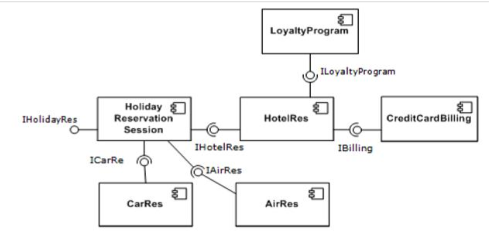
\includegraphics[scale=0.5]{softwareComponentExample.png}
	\caption{Software Components Example}
\end{figure}

In the work of \cite{componentDef} a component is defined as abstract, self-contained
packages of functionality performing a specific business function within a technology framework

This definition ascertains the fact that a software component is a well defined and independent software that gives it services using well defined interfaces.

Component-based software development is very well known and widely used as a methodology, which helps greatly in the re usability of software and reduces the cost of development significantly.

The primary role of CBSE is to direct making of software system as stitching of parts or components , development of the individual components as reusable entities and maintenance of the system developed with timely replacement of components.

%-------------------------------------------

\section{Proposed Work}
From the discussions above it is found that there are two approaches for faster and accurate software component retrieval from a software component library.First approach is indexing while creating and adding software components to library.This approach has the disadvantages that it will be cumbersome for migrating all the previously created software components to a new format of storing software components for indexing.It is also difficult to make changes upon.Second approach is reducing the search space for component search using the requirements given.\\

I will be following the approach of grouping together various components available into various clusters and generate a hierarchy of software component clusters.

Using the cluster headings of the hierarchy and requirements query text a subset of components for further searching is produced.This subset of components then needs to be compared one by and one and added to the output if it matches the component requirement.\\

For fine grained searching simple keyword and string matching is done on the functionality attribute of the component.each comparison will generate a similarity score and in the end the components identified will be displayed in decreasing order of the similarity score.
\subsection{Assumptions}
\begin{enumerate}
    \item The components available don't have external dependencies except language and library based dependency
    \item The components are properly maintained with all the attributes
    \item The requirements is very descriptive and giving language and type is a must
\end{enumerate}

\subsection{Working}
The overall objective is to create a hierarchy of cluster of software components based on similarity of attributes.The hierarchy created will helps in reducing the search space for searching of components.A hierarchical organization of reusable components that will provide a fast means for browsing, retrieving, and searching of software components.\cite{formal}.

\begin{figure}[t]
    \centering
    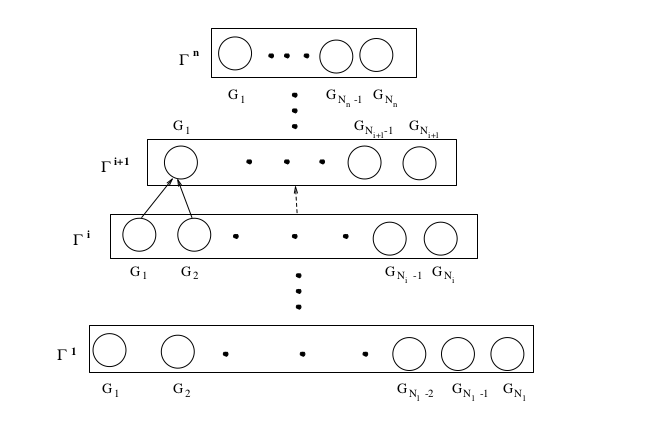
\includegraphics[scale=0.5]{agglomerativeClustering.png}
    \caption{Agglomerative Hierarchial Clustering}
    \label{fig:working}
\end{figure}

\begin{itemize}
    \item \textbf{Step 1: Data Preparation} The components available in the library are added by specifying attributes such as name,language,type,domain,visibility and functionality
    \item \textbf{Step 2: Similarity Calculation} For each component
    similarity is calculated with every other component based on the attributes language,type,domain and visibility.Functionality attribute will be used in later stage.The similarity is calculated by calculating adding the Levenshtein distance between the attribute values.Since less the distance more similar are the 2 values the distance is multiplied by -1 for proper ordering.

    \item \textbf{Step 3: Clustering} Agglomerative hierarchical clustering is a unsupervised learning algorithm.AHC algorithm is used on the software components using the similarity values.In each step of the algorithm two most similar components are grouped together and the similarity values are updated using the attribute values of this new merged component cluster.
    \item \textbf{Step 4: Keywords Generation} Once the hierarchy of clusters is ready the software component requirement is taken from user and the query is broken down into individual keywords using natural language processing by removing stop words ,duplicates and punctuation.
    \item \textbf{Step 5: Search Component Subset} The cluster headings and keywords generated are compared and the hierarchy is followed .The components for fine grained searching are added.
    \item \textbf{Step 6: Fine grained Searching} Functionality of all the search component subset is compared individually with the keywords.A similarity score is calculated based on the formula
    $number\;of\;keywords\;matched/number\;of\;words\;present\;in\; functionality$.All the components in the search component subset is displayed in decreasing order of the similarity score.
\end{itemize}

\subsection{Algorithms Used}
\begin{algorithm}[H]
        \SetAlgoLined
        \KwResult{one or more clusters}
        \Require \textbf{Input:} The set X = \{ x_1 , x_2 ,..,x_n \} \; and\;  the\; similarities\; s ( x_i , x_j ) , 1 \leq i,j \leq n \\
        \State Limit=1 ,N=n \\
        \For{1 \leq i,j \leq N , i \new j}
        {
            \state sim(G_i,G_j)=s(x_i,x_j)\\
        }
        \EndFor
        \While{ N \neq Limit}
        {
        \State N=N-1 \\
        Find pair of clusters $G_p$ and $G_q$ such that sim(G_p,G_q)=max \{ x \epsilon G_i,y \epsilon G_j \; s(x,y) \}\\
        update sim(G_i,G_j)\\
        }
        \caption{Component Clustering}\label{algo:3}
    \end{algorithm}
\section{Results and Discussion}

\section{Work Plan and Work Progress}

\subsection{Technology and Framework Used}
I have used Python to implement by hierarchical clustering.The dataset which contains components with attributes was prepared using spreadsheet program and stores as .csv file.Numpy array and pandas library was used using matrix.nltk library was used for natural language processing.

\subsection{Work Progress}
As of now clustering of components according to attribute values which are string values is performed which generates cluster headings based on the non matching attribute values.The searching of component is done directly by feeding the component requirement into the code.Fine grained searching used string comparison for generating similarity score.The overall results generated is not up to standard since the use is very limited and the generation of proper result is subject to proper query formation.using of string values to describe components inhibits in generating proper similarity scores and results.
\subsection{Future Work}
\begin{enumerate}
    \item Using formal method approach to describe software component
    \item developing the web application to enter proper requirement details
    \item using weights to some key requirements like language and domain
    \item develop a better fine grained search technique
    \item using a feedback rating option so as to prepare dataset for performing supervised learning
\end{enumerate}
\section{Conclusion}

% \section{References}
% \nocite{*}
% \bibliographystyle{plain}
% \bibliography{ref.bib}

\end{document}